\newpage
\section{Durchführung und Aufbau}
\label{sec:Durchführung}
Die Apparatur aus Abbildung \eqref{fig:Aufbau} wird mit einem elektronischen Zählwerk verbunden um die Impulszahl anzuzeigen. \\

\begin{figure}[H]
  \centering
  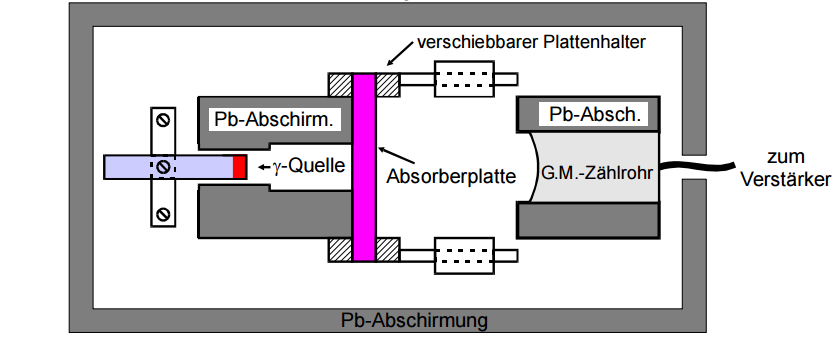
\includegraphics[height=7cm]{picture/Aufbau.PNG}
  \caption{Schematischer Aufbau um die Impulszahl von Strahlern zu messen. \cite[14]{sample}}
  \label{fig:Aufbau}
\end{figure}

Zu Beginn der Messung wird die Hintergrundstrahlung gemessen, indem 900\,s lang eine Messung ohne Strahler durchgeführt wird. Danach wird Caesium ($^{137}$Cs) als $\gamma$-Strahler in die Apparatur eingesetzt. Dann werden nacheinander 15 Kupferplatten und 20 Bleiplatten, mit unterschiedlicher Dicke, als Absorber eingesetzt. Bei jeder Dicke wird die Impulszahl mindestens 40\,s lang aufgenommen. Wenn die Impulszahl unter einen Wert von 250 fällt muss die Zählzeit so verlängert werden, das mehr als 250 Impulse regestriert werden. \\
Nun wird das Caesium durch Technetium ($^{99}$Tc) einem $\beta^-$-Strahler ersetzt. Hier werden allerdings 11 unterschiedlich dicke Aluminiumplatten verwendet. Außerdem wird mit einer Zählzeit von mindestens 100\,s begonnen und im Verlauf des Versuches weiter erhöht sodass die Impulszahl über einem Wert von 250 bleibt.
